%% Makros for Kompendium
%% 2023_11_19 philipp.freimann@bbw.ch

%% Die folgende Lösung habe ich hier angefragt:
%%https://tex.stackexchange.com/questions/701580/latex-equal-not-recognized-within-section-command
\ExplSyntaxOn
%% Text nur bei deutscher Sprache ausgeben:
\cs_new:Npn \deu #1 { \str_if_eq:eeT {\kLanguage}{deu} {#1} }
%% Text nur bei englischer Sprache ausgeben:
\cs_new:Npn \eng #1 { \str_if_eq:eeT {\kLanguage}{eng} {#1} }
\ExplSyntaxOff


%%%%%%%%%%%%%%%%%%%%%%%%%%%%%%%%%%%%%%%%%%%%%%%%%%%%%%%%%%%5
\newcounter{aufgabenNummer}
\setcounter{aufgabenNummer}{1}

%% see abvove
\ExplSyntaxOn
%% Text nur bei deutscher Sprache ausgeben:
\cs_new:Npn \isLoesungen #1 { \str_if_eq:eeT {\kLoesungen}{true} {#1} }
%% Text nur bei englischer Sprache ausgeben:
\cs_new:Npn \isAufgaben #1 { \str_if_eq:eeT {\kLoesungen}{false} {#1} }
\ExplSyntaxOff

%% see abvove
\ExplSyntaxOn
%% MatheNinja ausgeben:
\cs_new:Npn \printMatheNinja #1 { \str_if_eq:eeT {\kMatheNinja}{true} {#1} }
\ExplSyntaxOff

\newcommand{\kMatheNinjaLink}[2]{\printMatheNinja{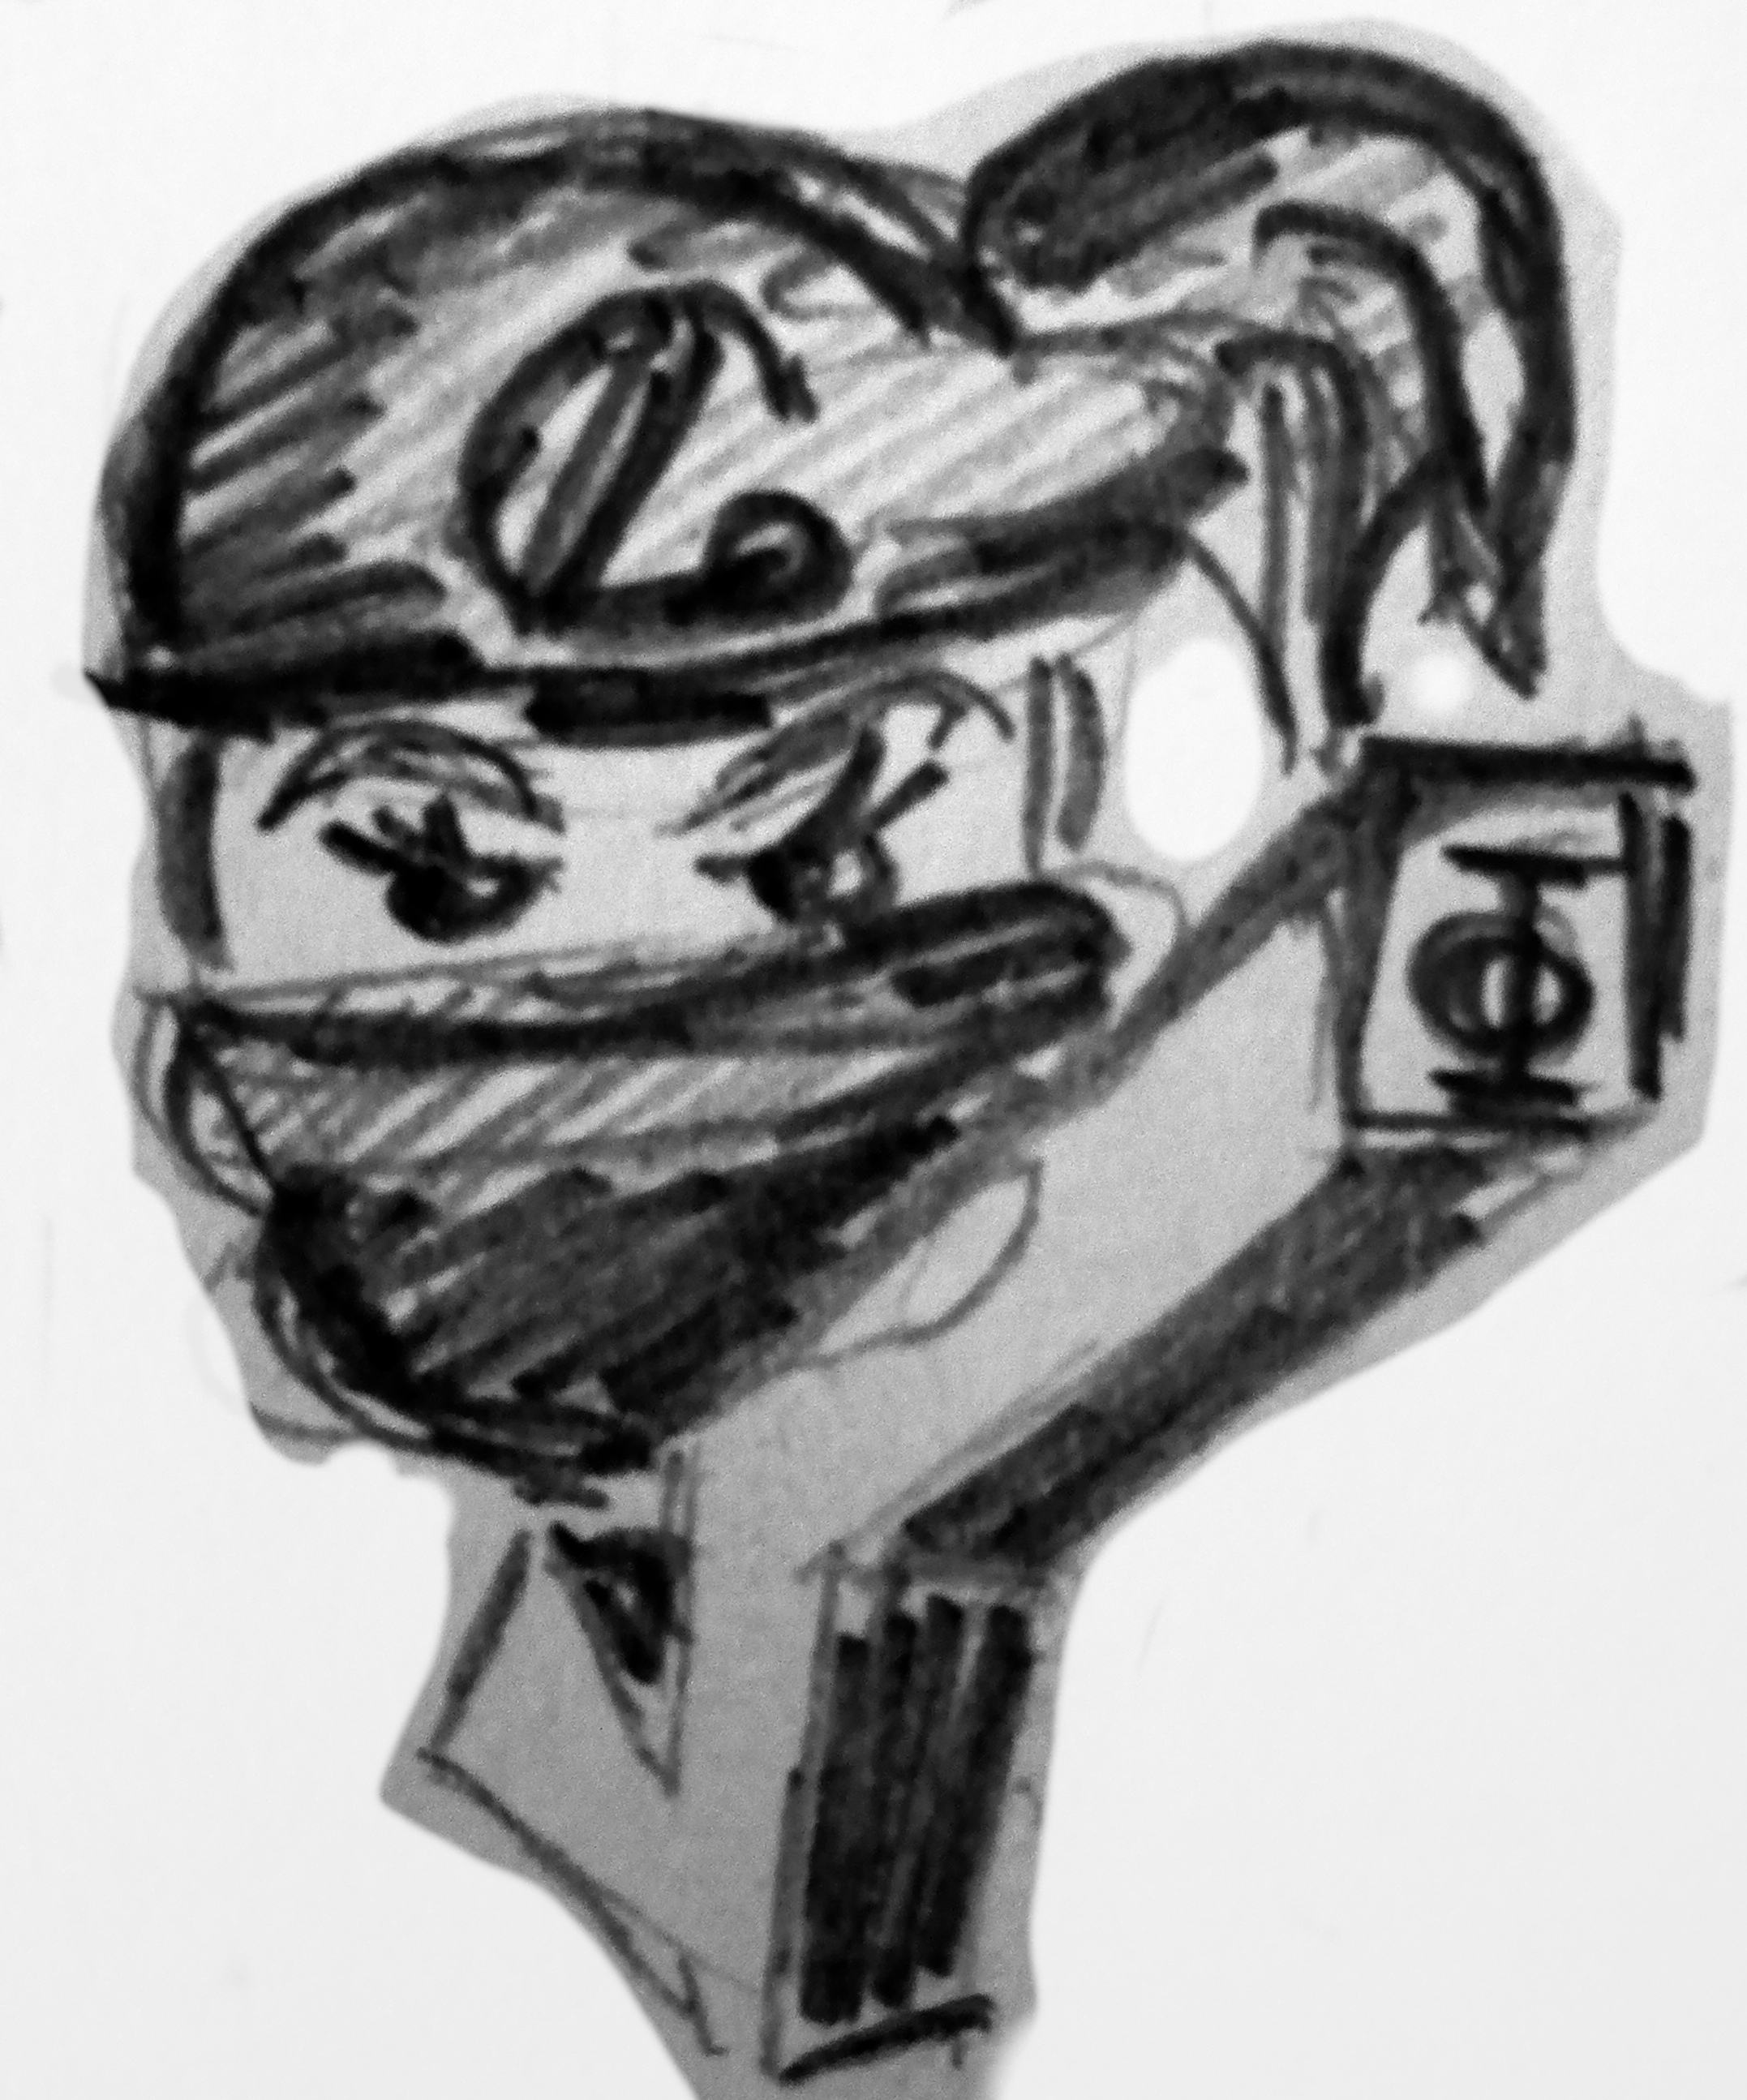
\includegraphics[width=15mm]{img/layout/matheninja.jpg} %%
%%«Mathe Ninja»
%%Link: \href{#2}{#1}\\(
\href{#2}{#2}
%)
\hrule}}

\newcommand{\mmPapierZwei}[2]{\begin{tikzpicture}
%%  \draw[step=4mm,bbwMMFarbe,ultra thin]
%%  \draw[step=4mm,bbwMMFarbe,thick]
  \draw[step=5mm,gray,line width=0.02mm]
  (0, 0) grid ({#2}, {#1});
\end{tikzpicture}}%%



\NewDocumentCommand{\isMMPapier}{m}{%%
  \ifthenelse{\equal{\kMMPapier}{true}}{%%
    
    \mmPapierZwei{#1}{17.5}

}{%%
}%% end ifthenelse
}%%


\NewDocumentCommand{\kPlatzFuerBerechnungen}{m}{%%
  \ifthenelse{\equal{\kMMPapier}{true}}{%%
    
    \mmPapierZwei{#1}{17.5}

}{%%
}%% end ifthenelse
}%%


%%\newcommand{\platzFuerBerechnungen}[1]{\isMMPapier{#1}}



\ExplSyntaxOn
%% Text nur bei Niveau BMP Ausgeben
\cs_new:Npn \nurNiveauBMP #1 { \str_if_eq:eeT {\kAufgabenNiveau}{nurBMP} {#1} }
%% Text nur bei englischer Sprache ausgeben:
\cs_new:Npn \auchTrainingsAufgabe #1 { \str_if_eq:eeT {\kAufgabenNiveau}{auchTraining} {#1} }
\ExplSyntaxOff




\ExplSyntaxOn
%% Text nur bei Niveau BMP Ausgeben
\cs_new:Npn \kVerweiseAltesKompendiumXX #1 { \str_if_eq:eeT {\kVerweiseAufsAlteKompendium}{true} {#1} }
\ExplSyntaxOff

%% Angabe \kVerweiseAltesKompendium 2018 {Seite}{Aufgabennummre}
\newcommand{\kVerweiseAltesKompendium}[2]{\kVerweiseAltesKompendiumXX{

\small{
\colorbox{gray!70}{
[Entspricht dem alten Kompendium (2018) Aufgabe #2 auf Seite: #1]
}%% end colornbox
}%% end small

}}%% end newcommand

%% Überschreiben mit "colorbox" o. ä.
\newcommand{\fragenMarkierung}{}

%% Kompendium Aufgaben
%% #1 : Aufgabentext
%% #2 : Lösungstext
%% #3 : Optional, 

%% Jedes Kapitel beginnt mit neuen Buchstaben.
%% Algebra hat Aufgabne A1, A2. ,,, Funktionen F1, F2, ...
%%
\newcommand{\kAufgabenBuchstabe}{0}
\newcommand{\kMetaAufgabe}[2]{%%
%  \kAufgabenBuchstabe{}\,\arabic{aufgabenNummer}. \fragenMarkierung{}:
\begin{minipage}{\textwidth}
\vspace{1mm}%%
  \fragenMarkierung{}\,\,%%
  \isLoesungen{{\color{blue}#2}}\isAufgaben{#1}
%%########################################################  \isMMPapier{#3}
\vspace{1mm}
\hrule{}%%
\end{minipage}%%  \vspace{2mm}
}%% end kaufgabe

\newcommand{\kNiveauAufgabe}[2]{%%
%%\nurNiveauBMP{\kMetaAufgabe{#1}{#2}{#3}}%%
\renewcommand{\fragenMarkierung}{\colorbox{orange!30}{\kAufgabenBuchstabe{}\,\arabic{aufgabenNummer}.(N)}}
\kMetaAufgabe{#1}{#2}%%
\stepcounter{aufgabenNummer}
}%% end kaufgabe

\newcommand{\kTrainingAufgabe}[2]{%%
\renewcommand{\fragenMarkierung}{\colorbox{blue!30}{\kAufgabenBuchstabe{}\,\arabic{aufgabenNummer}.(T)}}
\auchTrainingsAufgabe{\kMetaAufgabe{#1}{#2}}%%
\stepcounter{aufgabenNummer}
}%% end kaufgabe


\renewcommand{\indexname}{\deu{Stichwortverzeichnis}\eng{Index}}%%

\newcommand{\LoesungsMenge}{L}

\def\gleichungZZ#1#2#3#4{%%
  $$\left|
  \begin{array}{rcl}
    {#1} &=& {#2}\\
    {#3} &=& {#4}
    \end{array}\right|$$}%%

\def\gleichungDD#1#2#3#4#5#6{%%
  $$\left|
  \begin{array}{rcl}
    {#1} &=& {#2}\\
    {#3} &=& {#4}\\
    {#5} &=& {#6}\\
    \end{array}\right|$$}%%


%% Aufgaben die entfernt werden, können durchaus im Kompendium
%% Qulltext bleiben.

\newcommand{\entfernteAufgabe}[3]{... AUFGABE ENTFERNT ...}

\ExplSyntaxOn
%% Text nur bei Niveau BMP Ausgeben
\cs_new:Npn \kKommentar #1 { \str_if_eq:eeT {\kDraftKommentare}{true} {{\colorbox{red!10}{{\color{red} DRAFT: #1}}}} }
\ExplSyntaxOff



%% Zum Beispiel:
\newcommand{\zB}{z.\,B.}
